
\graphicspath{  {mainmatter/Hunt_2002/} }
\title*{2002: The importance of parameter mapping in electronic instrument design}
\titlerunning{Parameter Mapping in Electronic Instrument Design}

\author{Andy Hunt, Marcelo M. Wanderley and Matthew Paradis}
\authorrunning{Hunt et al.}

%\institute{Andy Hunt \at Music Technology Group, Electronics Department, University of York, Heslington, York YO10 5DD, \email {email adh2@york.ac.uk}
%\and Marcelo M. Wanderley \at Faculty of Music, McGill University 555, Sherbrooke Street West H3A 1E3---Montreal---Canada \email{mwanderley@acm.org}
%\and Matthew Paradis \at Music Technology Group, Music Department University of York, Heslington, York YO10 5DD \email{email mdjp100@york.ac.uk}}
%
%
\maketitle

\abstract*{In this paper we challenge the assumption that an electronic instrument consists
solely of an interface and a sound generator.  We emphasise the importance of the
mapping between input parameters and system parameters, and claim that this can
define the very essence of an instrument.}

\section{Electronic Instruments and the Mapping Layer}

In an acoustic instrument, the playing interface is inherently bound up with the
sound source.  A violin's string is both part of the control mechanism and the
sound generator.  Since they are inseparable, the connections between the two are
complex, subtle and determined by physical laws.  With electronic and computer
instruments, the situation is dramatically different.  The interface is usually a
completely separate piece of equipment from the sound source.  This means that
the relationship between them has to be defined.  The art of connecting these
two, traditionally inseparable, components of a real-time musical system (an art
known as \textit{mapping}) is not trivial.  Indeed this paper hopes to stress
that by altering the mapping, even keeping the interface and sound source
constant, the entire character of the instrument is changed.  Moreover, the
psychological and emotional response elicited from the performer is determined to
a great degree by the mapping.

\section{The Importance of Mapping}

In this section we emphasise the dramatic effect that the style of mapping can
have on ``bringing an interface to life.'' We focus on our own experience in
designing digital musical instruments and comment on several previous designs. An
extensive review of the available literature on mapping in computer music has
been presented by the authors in \cite{Hunt:2000b}, \cite{Wanderley:2001} and \cite{Wanderley:2002}.

\section{Informal Observations }

The first author has carried out a number of experiments into mapping.  The more
formal of these have been presented in detail in \cite{Hunt:2000} and \cite{Hunt:1999}, 
and are summarised later in this paper. Let us begin with some rather simple, yet interesting,
observations that originally sparked interest in this subject.  We have retained
the first person writing style to denote that these are informal, personal
reflections.

\subsection{The Accidental Theremin }

Several years ago I was invited to test out some final university projects in
their prototype form in the lab.  One of them was a recreation of a Theremin with
modern electronic circuitry.  What was particularly unusual about this was that a
wiring mistake by the student meant that the ``volume'' antenna only worked when
your hand was moving.  In other words the sound was only heard when there was a
rate-of-change of position, rather than the traditional position-only control. 
It was unexpectedly exciting to play.  The volume hand needed to keep moving back
and forth, rather like bowing an invisible violin.  I noted the effect that this
had on myself and the other impromptu players in the room.  Because of the need
to keep moving, it felt as if your own energy was directly responsible for the
sound.  When you stopped, it stopped.  The subtleties of the bowing movement gave
a complex texture to the amplitude.  We were ``hooked.''  It took rather a long
time to prise each person away from the instrument, as it was so engaging.  I
returned in a week's time and noted the irony that the ``mistake'' had been
corrected, deleted from the student's notes, and the traditional form of the
instrument implemented.

\subsection{Two Sliders and Two Sound Parameters }

The above observation caused me to think about the psychological effect on the
human player of ``engagement'' with an instrument.
To investigate this further I constructed a simple experiment. The interface for
this experiment consisted of two sliders on a MIDI module, and the sound source
was a single oscillator with amplitude and frequency controls.  In the first run
of the experiment the mapping was simply one-to-one, i.e. one slider directly
controlled the volume, and the other directly controlled the pitch (cf. Figure~\ref{Hunt:img-6}).

\begin{figure}[t]
\centering
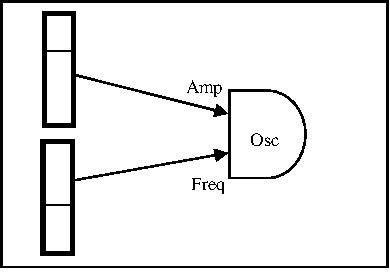
\includegraphics[width=70mm]{img-6-eps-converted-to-crop.pdf}
\caption{Simple mapping for Experiment 1}
\label{Hunt:img-6}       % Give a unique label
\end{figure}

I let several test subjects freely play with the instrument, and talked to them
afterwards.  In the second experimental run, the interface was re-configured to
emulate the abovementioned ``accidental Theremin.''  One slider needed to be moved
in order to make sound; the rate of change of movement controlled the
oscillator's amplitude.  But I decided to complicate matters (on purpose!) to
study the effect that this had on the users.  The pitch, which was mainly
controlled by the first slider, operated ``upside-down'' to most people's
expectations (i.e. pushing the slider up lowered the pitch).  In addition the
second slider (being moved for amplitude control) was used to mildly offset the
pitch---i.e. it was cross-coupled to the first slider  (cf. Figure~\ref{Hunt:img-2}).


\begin{figure}[t]
\centering
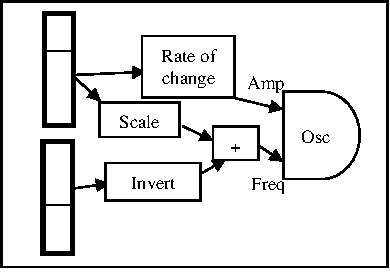
\includegraphics[width=70mm]{img-2-eps-converted-to-crop.pdf}
\caption{Complex mapping for Experiment 2}
\label{Hunt:img-2}       % Give a unique label
\end{figure}


A remarkable consistency of reaction was noted over the six volunteers who tried
both configurations.  With Experiment 1, they all commented within seconds that
they had discovered how the instrument worked (almost like giving it a mental
``tick''; ``yes, this is volume, and this is pitch'').  They half-heartedly tried to
play something for a maximum of two minutes, before declaring that they had
``finished.''  Problem solved.

With Experiment 2, again there was a noted consistency of response.  At first
there were grumbles.  ``What on earth is this doing?''  ``Hey---this is affecting
the pitch''  (implied cries of ``unfair,'' ``foul play'').  But they all struggled
with it---interestingly for several more minutes than the total time they spent
on Experiment 1.   After a while, their bodies started to move, as they developed
ways of offsetting one slider against the other, while wobbling the first to
shape the volume.  Nearly all the subjects noted that somehow this was rewarding;
it was ``like an instrument.''  Yet in both cases the interface (two sliders) and
the sound source (a single oscillator) were identical.  Only the mapping was
altered, and this had a psychological effect on the players.

\section{Mapping Experiments}

Several formal investigations have been carried out by the authors in order to
explore the essence and the effect of this mysterious mapping layer.

\subsection{Complex Mapping for Arbitrary Interfaces}

The first author carried out an investigation into the psychology and practicality of various interfaces for real-time musical performance \cite{Hunt:1999}.  The main part of this study took the form of major series of experiments to determine the effect that interface configuration had on the quality and accuracy of a human player's performance.  The details of the theory, experiments and results have been published \cite{Hunt:2000}.  They are summarised here, in order to give an overview of their implications for mapping strategies.

Three interfaces were used, and these are now described. The first interface (cf. Figure~\ref{Hunt:img-3}) represented a typical computer music editing interface with on-screen sliders connected one-to-one to each sound parameter. The second (cf. Figure~\ref{Hunt:img-4}) involved physical sliders (on a MIDI module) again connected in a one-to-one manner to the synthesis unit. The third interface (cf. Figure~\ref{Hunt:img-5}) consisted of a series of multi-parametric cross-mappings, and---like the accidental Theremin mentioned above---required constant movement from the user to produce sound.


\begin{figure}[t]
\centering
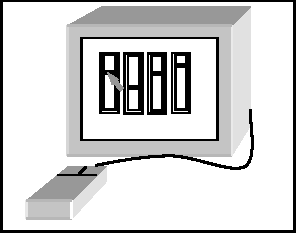
\includegraphics[width=70mm]{img-3-eps-converted-to-crop.pdf}
\caption{The ``mouse'' interface}
\label{Hunt:img-3}       % Give a unique label
\end{figure}



\begin{figure}[t]
\centering
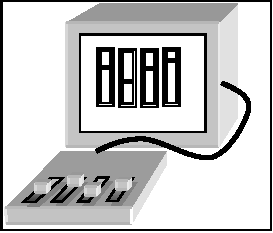
\includegraphics[width=70mm]{img-4-eps-converted-to-crop.pdf}
\caption{The ``sliders'' interface}
\label{Hunt:img-4}       % Give a unique label
\end{figure}



\begin{figure}[t]
\centering
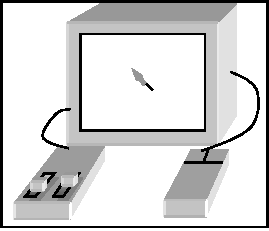
\includegraphics[width=70mm]{img-5-eps-converted-to-crop.pdf}
\caption{The `multi-parametric' interface}
\label{Hunt:img-5}       % Give a unique label
\end{figure}


Users attempted to copy (using each interface) a series of sounds produced by the computer.  The accuracy of reproduction was recorded for each user, over several attempts, spread out over a number of weeks.  Results were gathered numerically, and plotted on a series of graphs to compare the effect---over time---of each interface.  These quantitative results can be summarised for the multiparametric interface as follows:

\begin{itemize}
	\item The test scores in general were much higher than those for the other two
interfaces, for all but the simplest tests.
	\item There was a good improvement over time across all test complexities.
	\item The scores got better for more complex tests!
\end{itemize}

This last result may seem rather counter-intuitive at first sight; that people
performed better on the harder tasks.  However, this brings into question the
definition of a `hard task.'  If an interface allows the simultaneous control of
many parameters, maybe it really is easier to perform the more complex tasks, and
harder to accurately isolate individual parameters.

A range of qualitative results was also gathered by interviewing the test
subjects to establish their subjective experience of using each interface.  They
all concluded that the ``mouse'' interface was the most limited---as they could see
how impossible it would be to operate more than one parameter simultaneously. 
Surprisingly perhaps, they were nearly all extremely frustrated and angered by
the 4 physical sliders.  Comments abounded such as ``I should be able to do this,
technically, but I can't get my mind to split down the sound into these 4 finger
controls.''  Some users actually got quite angry with the interface and with
themselves.  The multi-parametric interface, on the other hand, was warmly
received---but not at the very beginning.  At first it seemed counter-intuitive
to most users, but they rapidly warmed to the fact that they could use complex
gestural motions to control several simultaneous parameters without having to
``de-code'' them into individual streams.  Many users remarked how ``like an
instrument'' it was, or ``how expressive'' they felt they could be with it.

\subsection{Focusing on the Effect of Mapping Strategies}

In the above experiment several factors may have affected the results.  For
instance, the multiparametric interface used cross-coupled parameters in addition
to the user's energy. It also decreased reliance on visual feedback, and provided
two-handed input, all of which may have contributed in varying degrees to the
interface's effectiveness.  An additional experiment was subsequently carried out
by the third author to focus entirely on the user's reaction to a change in
mapping strategy.

These tests utilised three contrasting mapping strategies, with a fixed user
interface and synthesis algorithm. The mappings were;

\begin{enumerate}
	\item simple one-to-one connections between input and output,

	\item one-to-one requiring the user's energy as an input.  This was implemented by
requiring the user to constantly move one of the sliders in a ``bowing''-like
action

	\item many-to-many connections from input to output, but also requiring the user's 
energy as in b).

\end{enumerate}

These mappings were used to control the parameters of a stereo FM synthesis
algorithm, including amplitude, frequency, panning, modulation ratio and
modulation index. The input device used was a MIDI fader box.  Users were asked
to play with each interface until they felt they had a good sense of how to
`drive it' to perform musical gestures.  No time limit was given to this process;
the users were encouraged to explore the possibilities of each set-up.  Data was
collected on the users' (subjective) views on the comparative expressivity and
learnability of each mapping and the accuracy of musical control that could be
achieved.

Whilst experimenting with the first mapping test (one-to-one) many users noted
that the simple division of parameters was not very stimulating. Users tended to
learn the parameter associations very quickly but then struggle to achieve any
improvement in their performance or expressive output.

The second test generated a range of comments, which suggested that the process
of injecting energy into a system presented a much more natural and engaging
instrument.  However, due to the proximity of sliders on the interface they found
it difficult to control other sliders whilst providing the required ``bowing''
action.  However, this problem lessened over time as the user practised.

The third and final user test (many-to-many mappings) provided some interesting
results.  Most of the test subjects noted that the appeal of this instrument was
that it was not instantly mastered but required effort to achieve satisfactory
results.  The instrument presented a challenge to the user, as one would expect
from a traditional expressive instrument.

These tests highlighted the differences between a general-purpose interface,
(such as the mouse) which has simple mappings but allows the user to begin
working instantly, and an interface with more complex mappings which must be
practised and explored in order to achieve truly expressive output.

\subsection{Learning from Acoustic Instruments}

In \cite{Rovan:1997} the second author and collaborators discussed the fact that by altering
the mapping layer in a digital musical instrument and keeping the interface (an
off-the-shelf MIDI controller) and sound source unchanged, the essential quality
of the instrument is changed regarding its control and expressive capabilities.

Previous studies, notably by Buxton \cite{Buxton:1986}, presented evidence that input devices
with similar characteristics (e.g. number of degrees of freedom) could lead to
very different application situations depending on the way these characteristics
were arranged in the device. In that study, however, the devices were not exactly
the same mechanically (one had two separate controllers and the other one
two-dimensional controller), so the situation is not the same as when using the
same input device with different mapping strategies, even if the results are
similar.

In \cite{Rovan:1997}, a Yamaha WX7 wind controller was used as the input device, and sound
was generated using additive synthesis models of clarinet sounds in IRCAM's FTS
environment (later in jMax).

The idea behind the project was simple: many wind instrument performers
complained that MIDI wind controllers tend to lack expressive potential when
compared to acoustic instruments such as the clarinet or saxophone.  A common
path to solving this problem involves improving the design of the controller by
adding extra sensors.  However, it was decided to challenge this assumption and
to solely work on the mapping layer between the controller variables and the
synthesis inputs (for a complete description see \cite{Rovan:1997}).

Another point became clear in this process: even if the WX7 was a faithful model
of a saxophone providing the same types of control variables (breath, lip
pressure and fingering), these variables worked totally \textit{independently} in
the MIDI controller, whereas they are \textit{cross-coupled} in acoustic
single-reed instruments. This natural cross-coupling is the result of the
physical behaviour of the reed, and since the equivalent ``reed'' in the
controller was a plastic piece that did not vibrate, and moreover was not coupled
to an air column, variables were simply independent.

Based on these decisions and facts, the authors proposed different mappings
between the WX7 variables and the synthesis parameters.  The first was basically
a one-to-one relationship, where variables were independent.  The second was a
model where the ``virtual airflow'' through the reed (loudness) was a function of
both the breath and lip pressure (embouchure), such as in an acoustic instrument.
 The third was a model that took into account both the ``virtual airflow'' and
the relationship between spectrum content to breath and embouchure; a model that
would match even more closely the real behaviour of the acoustic instrument.

Using these three different models, the system was performed by different
musicians and non-musicians. Results indicated that wind instrument performers
tended to stick with complex cross-coupled mappings similar to the single reed
behaviour (the third mapping strategy used), whereas beginners initially
preferred simpler mappings (easier to play and produce stable sounds).


\begin{figure}[t]
\centering
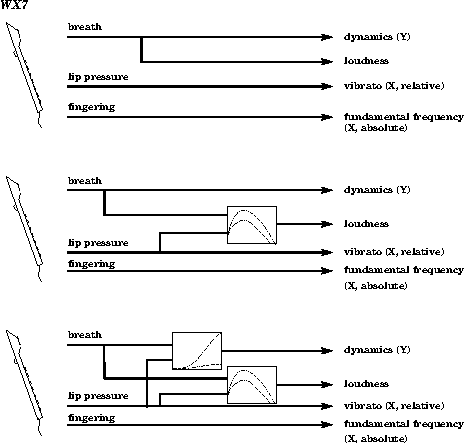
\includegraphics[width=\textwidth]{img-1-eps-converted-to-crop.pdf}
\caption{Several mappings used in the clarinet simulation presented in
 \cite{Rovan:1997}.}
\label{Hunt:img-1}       % Give a unique label
\end{figure}


The two most important consequences of this work were:

\begin{itemize}
	\item By just changing the mapping layer between the controller and the synthesis
algorithm, it was indeed possible to completely change the instrumental behaviour
and thus the instrument's feel to the performer. Depending on the performer's
previous experience and expectations, different mappings were preferred.

\item By deconstructing the way that the reed actually works, it was noted that the
choice of mapping could be important as a pedagogical variable. Indeed, in stark
contrast with acoustic instruments where the dependencies between parameters are
unchangeable, cross-coupling between variables can easily be created or destroyed
in digital musical instruments. This means that performers could focus on
specific aspects of the instrument by explicitly defining its behaviour. Possible
options could include:

\begin{itemize}
	\item complex (cross-coupled) control of loudness with one-to-one control of timbre,
	\item one-to-one loudness and complex timbre controls, or,
	\item complex loudness and timbre controls, such as in the real instrument.
\end{itemize}

\end{itemize}


Even if these results supported the essential role of mapping (and the
importance of devising mapping strategies other than one-to-one during the design
of digital musical instruments), they could not be easily extrapolated to more
general situations. In fact, in the above specific case, there \textit{did exist}
a model of complex mapping to be followed, since the controller was a model of
the acoustic instrument. So what about mappings in general digital musical
instruments using alternate controllers, those not based on traditional acoustic
instruments?

\section{Models and Guidelines For Mapping}

Since there will not always be ready models for inspiration when designing
mapping strategies for new digital musical instruments, the task then becomes one
of proposing guidelines for mapping and also, if possible, devising models that
can facilitate the implementation of mapping strategies other than simple
one-to-one relationships.

In trying to answer this question of how to extend a specific mapping solution
to a more general case, a model of mapping for digital musical instruments was
proposed in \cite{Wanderley:1998}.  It was based on the separation of the mapping layer into two
independent layers, coupled by an intermediate set of user-defined (or
``abstract'') parameters. This model was presented in the framework of a set of
extensions to jMax later known as ESCHER (actually, a set of objects developed by
Norbert Schnell to perform interpolation using additive models).

This idea is based on previous works, such as those of Mulder et al. \cite{Mulder:1997},
M\'{e}tois \cite{Metois:1996}, and Wessel \cite{Wessel:1979}. A similar direction was presented by Mulder and
Fels in \cite{Mulder:1998a} and later by Garnett and Goudeseune \cite{Garnett:1999}. Basically, all these works
have used higher levels of abstraction as control structures instead of raw
synthesis variables such as amplitudes, frequencies and phases of sinusoidal
sound partials. The main point made in \cite{Wanderley:1998} was to explicitly think about two
separate mapping layers and the strategies to implement these, and not on the
choice of intermediate parameters themselves, whether perceptive, geometrical or
``abstract'' \cite{Wanderley:1999}.

The intrinsic advantage of this model is its flexibility. Indeed, for the same
set of intermediate parameters and synthesis variables, the second
mapping layer is independent of the choice of controller being used. The same
would be true in the other sense: for the same controller and the same set of
parameters, multiple synthesis techniques could be used by just adapting
the second mapping layer, the first being held constant. Specifically in this
case, the choice of synthesis algorithm is transparent for the user

The original two-layered model has recently been expanded to include three
mapping layers in two independent performance works by Hunt and Myatt (RIMM The Real-time Interactive MultiMedia project, and
by Arfib and collaborators \cite{Arfib:2002}.  These works support the idea that, by using
multi-layered mappings, one can obtain a level of flexibility in the design of
instruments and that moreover, these models can indeed accommodate the control of
different media, such as sound and video, in a coherent way.

\subsection{One-to-one Mappings---Multiple Layers}

We have noted that there is a tendency for designers to make one-to-one mappings
when constructing an interface.  We can \textit{use} this tendency to improve the
mapping process if we utilise the many layered models outlined above.  The
following scenario may illustrate this:

Imagine a system whose interface inputs included `button 1,' `button 2,'  `slider
1,' `slider 2,' `mouse x,' and `mouse y.'  Let us suppose that the synthesis system
was a Frequency Modulation module with inputs such as `carrier frequency,'
`carrier amplitude,' `modulation frequency' etc.  Now consider the two
possibilities below:

	
\begin{description}
\item[Case 1:] let us consider a designer working to connect the above inputs
to the above outputs.  We are quite likely to see arbitrary connections such as 
``mouse x controls carrier frequency,'' and ``slider 1 controls modulation
frequency.''  These give us the oft-encountered one-to-one mappings.

\item[Case 2:] let us imagine that a mapping layer has already been devised to
abstract the inputs to parameters such as `energy,' `distance between sliders,'
`wobble' etc.  Also let us imagine that there is a mapping layer before the FM
synthesis unit, providing higher-level control inputs such as `brightness,'
`pitch,' `sharpness' etc.  Now we can picture the designer making a relationship
such as ``energy controls brightness.''  On the surface this may appear to be yet
another one-to-one mapping.  Indeed it is---at the conceptual level. 
However, when you consider how `energy' is calculated from the given inputs, and
how `brightness' has to be converted into the FM synthesis primitives, you will
notice how many of the lower-level parameters have been cross-coupled.

\end{description}


Thus the many-level mapping models are a way of simplifying the design process,
and of helping the designer to focus on the final effect of the mapping, as well
as providing a convenient method of substituting input device or synthesis
method.

\section{Future Discussion of Mapping}

From the evidence presented above in both informal and controlled experiments,
there is definitely a need to come up with better-designed mappings than simple
(engineering style) one-to-one relationships. General models of mappings have
been proposed and expanded to incorporate multimedia control, but also to fit
several levels of performance, from beginners to highly skilled players.

One attempt to foster the discussion in this direction has been initiated in the
context of the ICMA/EMF Working Group on Interactive Systems and Instrument
Design in Music. % \cite{:2000b}. 
A further effort is currently being carried out in the form
of a special issue on ``Mapping Strategies for Real-time Computer Music''
guest-edited by the second author \cite{Wanderley:2002} to appear as volume 7, number 2 of the
journal Organised Sound later this year.

We therefore welcome comments and criticism on issues related to mapping so as
to push the discussion on this essential---although often ignored---topic.

\section{Conclusions}

The mapping `layer' has never needed to be addressed directly before, as it has
been inherently present in acoustic instruments courtesy of natural physical
phenomena.  Now that we have the ability to design instruments with separable
controllers and sound sources, we need to explicitly design the connection
between the two.  This is turning out to be a non-trivial task.

We are in the early stages of understanding the complexities of how the mapping
layer affects the perception (and the playability) of an electronic instrument by
its performer.  What we know is that it is a very important layer, and one that
must not be overlooked by the designers of new instruments.



\section*{Author Commentary: Reflections on Parameter Mapping in Electronic Instrument Design}

\paragraph{Andy Hunt and Marcelo M. Wanderley}


In the 80's and early 90's many papers were published on the development of digital musical instruments (DMIs) and interfaces for musical expression, mostly at conferences such as the International Computer Music Conference (ICMC) and in the Computer Music Journal, both starting in the mid-late 70s. A number of amazing instruments and methods were proposed, many of them subsequently summarized in the book ``New Digital Musical Instruments: Control and interaction beyond the keyboard'' \cite{Miranda:2006}. These papers mostly presented novel interfaces and/or sound synthesis methods for musical control, but few specifically
addressed the issues involved in how to map interface outputs to synthesis inputs. One-to-one arbitrary mappings were the norm, but notable exceptions included the works of Ian Bowler et al. (ICMC1990), Michael Lee and David Wessel (ICMC1992), Insook Choi et al. (ICMC1995), Stuart Favilla (ICMC1996) and Axel Mulder et al. (Workshop Kansei 1997).

This NIME 2002 paper arose from a collaboration between Andy Hunt and Marcelo Wanderley (with Matthew Paradis, a D.Phil. student of Hunt) in the late 90's and early 2000's. Both researchers were among the first to study and begin to formalize the role of mapping in digital musical instruments (DMIs). In this paper, the questions we tackle are as follows: What if more complex strategies are used instead of one-to-one mappings, such as what happens in many acoustic musical instruments? How can one make sense of the various mapping possibilities in DMIs (e.g. implicit, explicit)? What is the influence of the choice of mapping on DMI design/performance?


Wanderley started to look at the importance of mapping in DMI design in 1997, when in collaboration with Butch Rovan, Shlomo Dubnov and Philippe Depalle he presented a paper at the International Workshop on ``Kansei, The Technology of Emotion,'' organized by Antonio Camurri in Genoa, Italy. In 1998, in collaboration with Norbert Schnell and Butch Rovan, he published a sequence paper on mapping strategies in the software application ``Escher,'' developed at IRCAM. In this paper, the notion of mapping layers was proposed to formalize and articulate the definition of mapping strategies.


At the same time, Hunt was working on his D.Phil. thesis also on mapping, under the supervision of Ross Kirk at the University of York, UK. His work was the first (and up to now possibly the only one) to have looked at the long-term performance with different mapping strategies. Apart from this major contribution, the main difference between these works was that, while Wanderley et al. were inspired by a known mapping model (that of a clarinet), Hunt and Kirk dealt with arbitrary mapping choices (i.e. with no known models to base the mapping on).


In 1999, through the project CUIDAD, organized by IRCAM and with the participation of the University of York, both had the opportunity to collaborate in joining their respective work on mapping. A first result was a paper published at ICMC 2000 in Berlin \cite{Hunt:2000b}. They continued to work on this topic through a few more papers, including the one in NIME 2002. One for Organised Sound and one for the Journal of New Music Research, directly derived from the NIME 2002 paper. Altogether, these papers were cited more than 500 times (Google Scholar, Sept 28 2015).


One interesting issue arose at the conference, held at the former Media Lab Europe, in Dublin, Ireland. One of the keynote speakers was interactive music pioneer Joel Chadabe, who gave a talk with the title ``The Limitations of Mapping as a Structural Descriptive in Electronic Instruments,'' a very interesting contrast to the title we proposed (``The importance of Parameter Mapping in Electronic Instrument Design''). This is mostly due to the notion of an ``electronic instrument,'' a reactive device in Hunt and Wanderley's view, but an ``interactive system'' in Chadabe's (see Bert Bongers definition of interactive and reactive systems \cite{Bongers:2000}).

Since then, Wanderley has edited (or co-edited) two special journal editions on Mapping in DMIs (Organised Sound vol. 7, 2002, and recently in the Computer Music Journal, vol. 38, 2014, with Joseph Malloch) and published a few more works focusing on mapping. Hunt has created and made several contributions to the field of ``interactive sonification,'' mostly in collaboration with Thomas Hermann (University of Bielefeld).

While much has been done since the paper was first written, mapping is still an open field of research,  mostly in terms of tools to help define mapping strategies in DMIs (see \cite{Wanderley:2014} for updated information). Work is still needed to understand the implications of mapping choices in short and long-term performance with DMIs.


\section*{Expert Commentary: Listen to the Inner Complexities}

\paragraph{Doug Van Nort}

Fairly early in the development of interactive computer music, people had already been thinking about user manipulation of all facets of digital sound, with a major early voice in this area being David Wessel through his idea of timbre space as a musical control structure \cite{Wessel:1979}. By the late 90's and early 2000's, ever-increasing processing speeds had allowed for high-quality sound synthesis to run in real-time. This led to an explosion in research on input devices and sensor technologies for expressive control of these various sound creation algorithms, moving beyond the limiting standard of the MIDI keyboard. 

As research raced forward in the areas of real-time sound synthesis and sensor-based controllers, a group of researchers rightly recognized that all of the essential algorithmic decisions that associate control input with sound output---the area of mapping---was being overlooked. They looked towards the more mature field of Human Computer Interaction (HCI) for inspiration, and the work of researchers such as William Buxton in order to more fully understand the ergonomic and psychological influence that simply changing a mapping can have on a user, or in this case performer. 

The article by Hunt, Wanderley and Paradis is particularly important as it represents the coming together of two early research streams. Hunt's and Wanderley's respective dissertation projects and subsequent research are two of the earliest to tackle this area of inquiry, as is well represented in the ``Trends in Gestural Control of Music'' collection \cite{:2000c} as well as a special issue of Organised Sound \cite{Wanderley:2002}. 

This NIME 2002 article serves two key purposes: the first is that it gives an important brief introduction to these preceding projects; the second is that it attempts to establish and articulate the importance of mapping by formally exploring this through quantitative and qualitative user studies. While one could level a fair criticism by noting that the studies presented lack the depth and methodological rigor of many found within the world of HCI, the fact remains that this work opened up the question of how the ostensibly simple act of control-to-sound parameter associations could profoundly impact the ``feel'' of the digital musical instrument. Various works have followed up on this early research including my own dissertation \cite{Van-Nort:2010}, largely devoted to expanding this conversation on the topic of mapping. 

Certainly not all members of the NIME community have agreed with the approach of the 2002 Hunt et al. work: some maintain that mapping is purely an artistic decision of the composer/designer, while others maintain the spirit of this article, that it is an essential determinant of expressivity for any performer who comes into contact with a given digital musical instrument. My personal view is that, as with most things, the truth lies somewhere in between and both are correct depending on the musical intent. If we are talking about a complex interactive system that a performer is simply guiding, then perhaps mapping is even a limiting concept, as proposed by Chadabe \cite{Chadabe:2002}. However, if we are talking about the continuous shaping of sonic activity with a goal of achieving nuanced control and expression that rivals acoustic instrumental practice, then this question of ``what to map where'' and how various control signals are extracted, gated, associated, adapted, conditioned, etc. can have profound impact on a digital performer's ability to keep up with their analog musical vision. 

This article has played no small role in opening up this conversation in the context of the NIME community. As we move forward with ever more sophisticated techniques of machine learning at our disposal, I hope that future NIME creators will remember the profound influence that can be wrought by a subtle change in transfer function, interpolation method, or cross-coupling of parameters, and that one should take time to listen to the inner complexities of their system's behaviour with their musical ears, mind and body. Further to this point, I strongly suggest that freezing the instrumental system's state and deeply engaging with performance in a variety of improvised contexts will present the true challenges and roadblocks to one's performative voice. It may be that a new method of gestural sensing or sonic output is required, but do not overlook the gesturality and dynamism inherent in the small choices that lie in between.  
